The following is the block diagram of a hierarchical control system with two nested feedback loops. Simplify the block diagram to find the transfer function $\frac{Y(s)}{R(s)}$.

\begin{center}
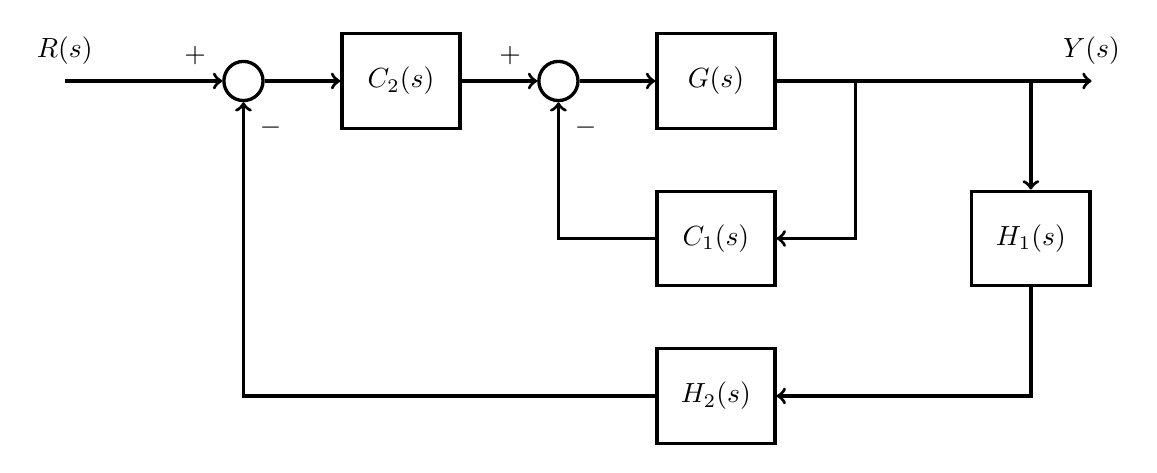
\begin{tikzpicture}[very thick,
sysblock/.style={draw,rectangle,inner sep=6pt,minimum width=1.5cm,minimum height=1.2cm,very thick},
delayblock/.style={draw,rectangle,inner sep=6pt,minimum width=0.5cm,minimum height=1.0cm,very thick},
node/.style={fill,inner sep=0pt,outer sep=0pt},
summer/.style={circle,draw,very thick,inner sep=5pt}]

\draw (-4,0) node[summer] (sum2) {};
\draw (-2,0) node[sysblock] (C2) {$C_{2}(s)$};
\draw (0,0) node[summer] (sum) {};
\draw (2,0) node[sysblock] (G) {$G(s)$};
\draw (2,-2) node[sysblock] (C1) {$C_{1}(s)$};
\draw (6,-2) node[sysblock] (H1) {$H_{1}(s)$};
\draw (2,-4) node[sysblock] (H2) {$H_{2}(s)$};


\draw[<-] (sum2.180) node[above left=2pt] {$+$} -- ++(-2,0) node[above=2pt] {$R(s)$};
\draw[->] (sum2.0) -- (C2.180);
\draw[->] (C2.0) -- (sum.180) node[above left=2pt] {$+$};
\draw[->] (sum.0) -- (G.180);
\draw[->] (G.0) -- ++(4,0) node[above=2pt] {$Y(s)$};
\draw[->] (G.0) ++(1,0) |- (C1.0);
\draw[->] (G.0 -| H1.90)  -- (H1.90);
\draw[->] (H1.-90) |- (H2.0);
\draw[->] (H2.180) -| (sum2.-90) node[below right=2pt] {$-$};
\draw[->] (C1.180)  -| (sum.-90) node[below right=2pt] {$-$}; 
\end{tikzpicture}
\end{center}

